\chapter{The structural flexibility of \protein{Mad1} facilitates the coupling between \protein{Mad2}'s conformational change and the assembly of the mitotic checkpoint complex (MCC)}
\label{chpt:4}

In previous chapters, we presented evidence on the cooperativity among multiple MELT motifs on the same \protein{Knl1} phosphodomain (the first layer in the SAC signaling cascade). This phenomenon is probably explained by SAC proteins that concurrently bind to these MELT motifs in close spatial proximity (the second layer). In this chapter, we will focus on the spatio-temporal coupling scaffolded by \protein{Mad1} between \protein{Mad2}'s conformational change and the assembly of the MCC \cite{BUB1-CDC20-MAD1,Tripartite} (note that as mentioned in \myref{CoreSAC}, ``\protein{Mad1}'' here and in many other instances throughout this chapter refers to the \protein{Mad1}-\protein{Mad2} heterotetramer). We term it ``the third layer'' in the SAC signaling cascade. % As mentioned in \myref{Chapter3Discussions}, \protein{Mad1} can be recruited to signaling kinetochores by multiple pathway.

The formation of the \protein{Cdc20}-\protein{Mad2} dimer, an MCC subcomplex, is considered to be the rate-limiting step in the assembly of the MCC based on an \Latin{in vitro} study \cite{Faesen2017}. However, how \protein{Cdc20}-\protein{Mad2} dimerization is catalyzed in the cell was unclear for a long time. Critical studies published later showed that locking cytosolic \protein{Mad2} to the closed conformation inhibited the dimerization between \protein{Cdc20} and \protein{Mad2} and compromised the SAC signaling activity \cite{Ma+Poon2016,Ma+Poon2018,Kim2018}. These findings hinted that the conformational change of \protein{Mad2} and \protein{Cdc20}-\protein{Mad2} dimerization might be temporally coupled. In 2021, two papers published back-to-back (based on either \Latin{in vitro} reconstitution \cite{BUB1-CDC20-MAD1} or studies in \Latin{C. elegans} \cite{Tripartite}) presented evidence supporting the cooperative binding of \protein{Cdc20} to signaling kinetochores and the spatio-temporal coupling between \protein{Mad2}'s conformational change and the formation of the \protein{Cdc20}-\protein{Mad2} dimer (see \myref{TwoModels}), which offered critical molecular insight into the synergy in this process.

In this chapter, we approached the suggested spatio-temporal coupling from a different angle -- by looking into the role of the conserved structural flexibility of \protein{Mad1} in the catalysis of \protein{Cdc20}-\protein{Mad2} dimerization. We began this hypothesis-driven study independently in 2018, which has evolved into a collaboration project. I am the sole contributor to most cell biology data here. Simon Han performed preliminary tests on the feasibility and physiological activity of internally tagged Mad2p in the budding yeast. We took advantage of the free ColabFold advanced Jupyter Notebook (henceforth simply referred to as ``ColabFold advanced algorithm''), which implemented the tremendously successful, recently publicized structural prediction algorithm AlphaFold 2 in Google Colaboratory \cite{ColabFold, AlphaFold}. \Latin{In vitro} reconstitution results from our collaborators (Dr. Valentina Piano and Amal Alex from Dr. Andrea Musacchio's group at the Max Planck Institute of Molecular Physiology in Germany) will be mentioned to write a coherent story, but those data are not included here.

\section{The molecular mechanism of \protein{Cdc20}-\protein{Mad2} dimerization: the ``assembly line'' model \Latin{versus} the ``knitting'' model}
\label{TwoModels}

The formation of the \protein{Cdc20}-\protein{Mad2} dimer, an MCC subcomplex, is considered to be the rate-limiting step in the assembly of the MCC based on an \Latin{in vitro} study \cite{Faesen2017}. However, how \protein{Cdc20}-\protein{Mad2} dimerization is catalyzed in the cell was unclear for a long time. \protein{Cdc20} has a flexible N-terminal region with a \protein{Mad2}-interacting motif (MIM) and a C-terminal WD40 \textbeta{}-propeller fold \cite{hCDC20Structure} (in \myref{TwoModelCartoons}, the N- and C-terminal regions are represented by a light gray line and a light gray circle, respectively). \protein{Mad2} has three known conformations: the open conformation (denoted as O-\protein{Mad2} and illustrated as a magenta open lock with a circular body in \myref{TwoModelCartoons}), the intermediate conformation (denoted as I-\protein{Mad2} and illustrated as a peach open lock with a rectangular body in \myref{TwoModelCartoons}), and closed (denoted as C-\protein{Mad2} and illustrated as a red closed lock with a rectangular body in \myref{TwoModelCartoons}) \cite{I-MAD2}. A popular explanation of the catalytic mechanism of the switch of \protein{Mad2} from the open conformation to the closed conformation is the template model \cite{TemplateModel}. This model states that the conformational switch of \protein{Mad2} may be facilitated by the homodimerization between a closed \protein{Mad2} (bound to \protein{Mad1}'s MIM in the \protein{Mad1}-\protein{Mad2} heterotetramer) and the \protein{Mad2} that undergoes the conformational switch. C-\protein{Mad2} binds to \protein{Cdc20}, buckling the MIM of \protein{Cdc20} in a safety belt-like manner similar to how C-\protein{Mad2} binds to \protein{Mad1} \cite{Structure1GO4, SpMCC}. The \protein{Cdc20}-\protein{Mad2} dimer binds to \protein{BubR1}/\protein{BubR1}-\protein{Bub3} and forms the MCC.

\protein{Cdc20} binds to \protein{Mad1}'s C-terminal RING finger-containing proteins, WD repeat-containing proteins, and DEAD-like helicases (RWD) domain phosphorylated by \protein{Mps1} through BOX1, an N-terminal basic motif of \protein{Cdc20} \cite{Ji2017eLife, BUB1-CDC20-MAD1} (illustrated in \myref{TwoModelCartoons} as the contact between \protein{Cdc20}'s light gray N-terminal region and \protein{Mad1}'s dark green C-terminal domain). Given the spatial proximity between the catalytic site of \protein{Mad2}'s conformational switch and the MIM of \protein{Cdc20}, it is attractive to investigate the potential coupling between \protein{Mad2}'s conformational switch (\textcircled{\small{1}} in \myref{TwoModelCartoons}) and the binding between \protein{Cdc20} and \protein{Mad2} (\textcircled{\small{2}} in \myref{TwoModelCartoons}). Therefore, we set out to test two opposite models, which we named the ``assembly line'' model and the ``knitting'' model. As the names suggest, the ``assembly line'' model indicates that the two processes happen in two separate steps and newly switched \protein{Mad2} from step \textcircled{\small{1}} enters a free cytosolic pool and then participates in step \textcircled{\small{2}}, as if two steps in an assembly line mediated by a warehouse. In contrast, the ``knitting'' model indicates that like knitting, the two processes are closely coordinated in one step  (\Latin{i.e.}, \textcircled{\small{1}} is coupled to \textcircled{\small{2}}). The two regions of the \protein{Mad1}-\protein{Mad2} heterotetramer with known structures shown in the top panel of \myref{HsMAD1CTerStructure} function as the two knitting needles. They are connected by a region of unknown structure, which is predicted to be a flexible loop (see \myref{MAD1_MIM-RLK_Lupas+DeepCoil2}; this region is henceforth simply referred to as ``\protein{Mad1}'s loop region''). Interestingly, the primary sequence of this loop region is not well conserved from yeast to human, but the secondary structure is predicted to be conserved.

\begin{figure}
    \centering
    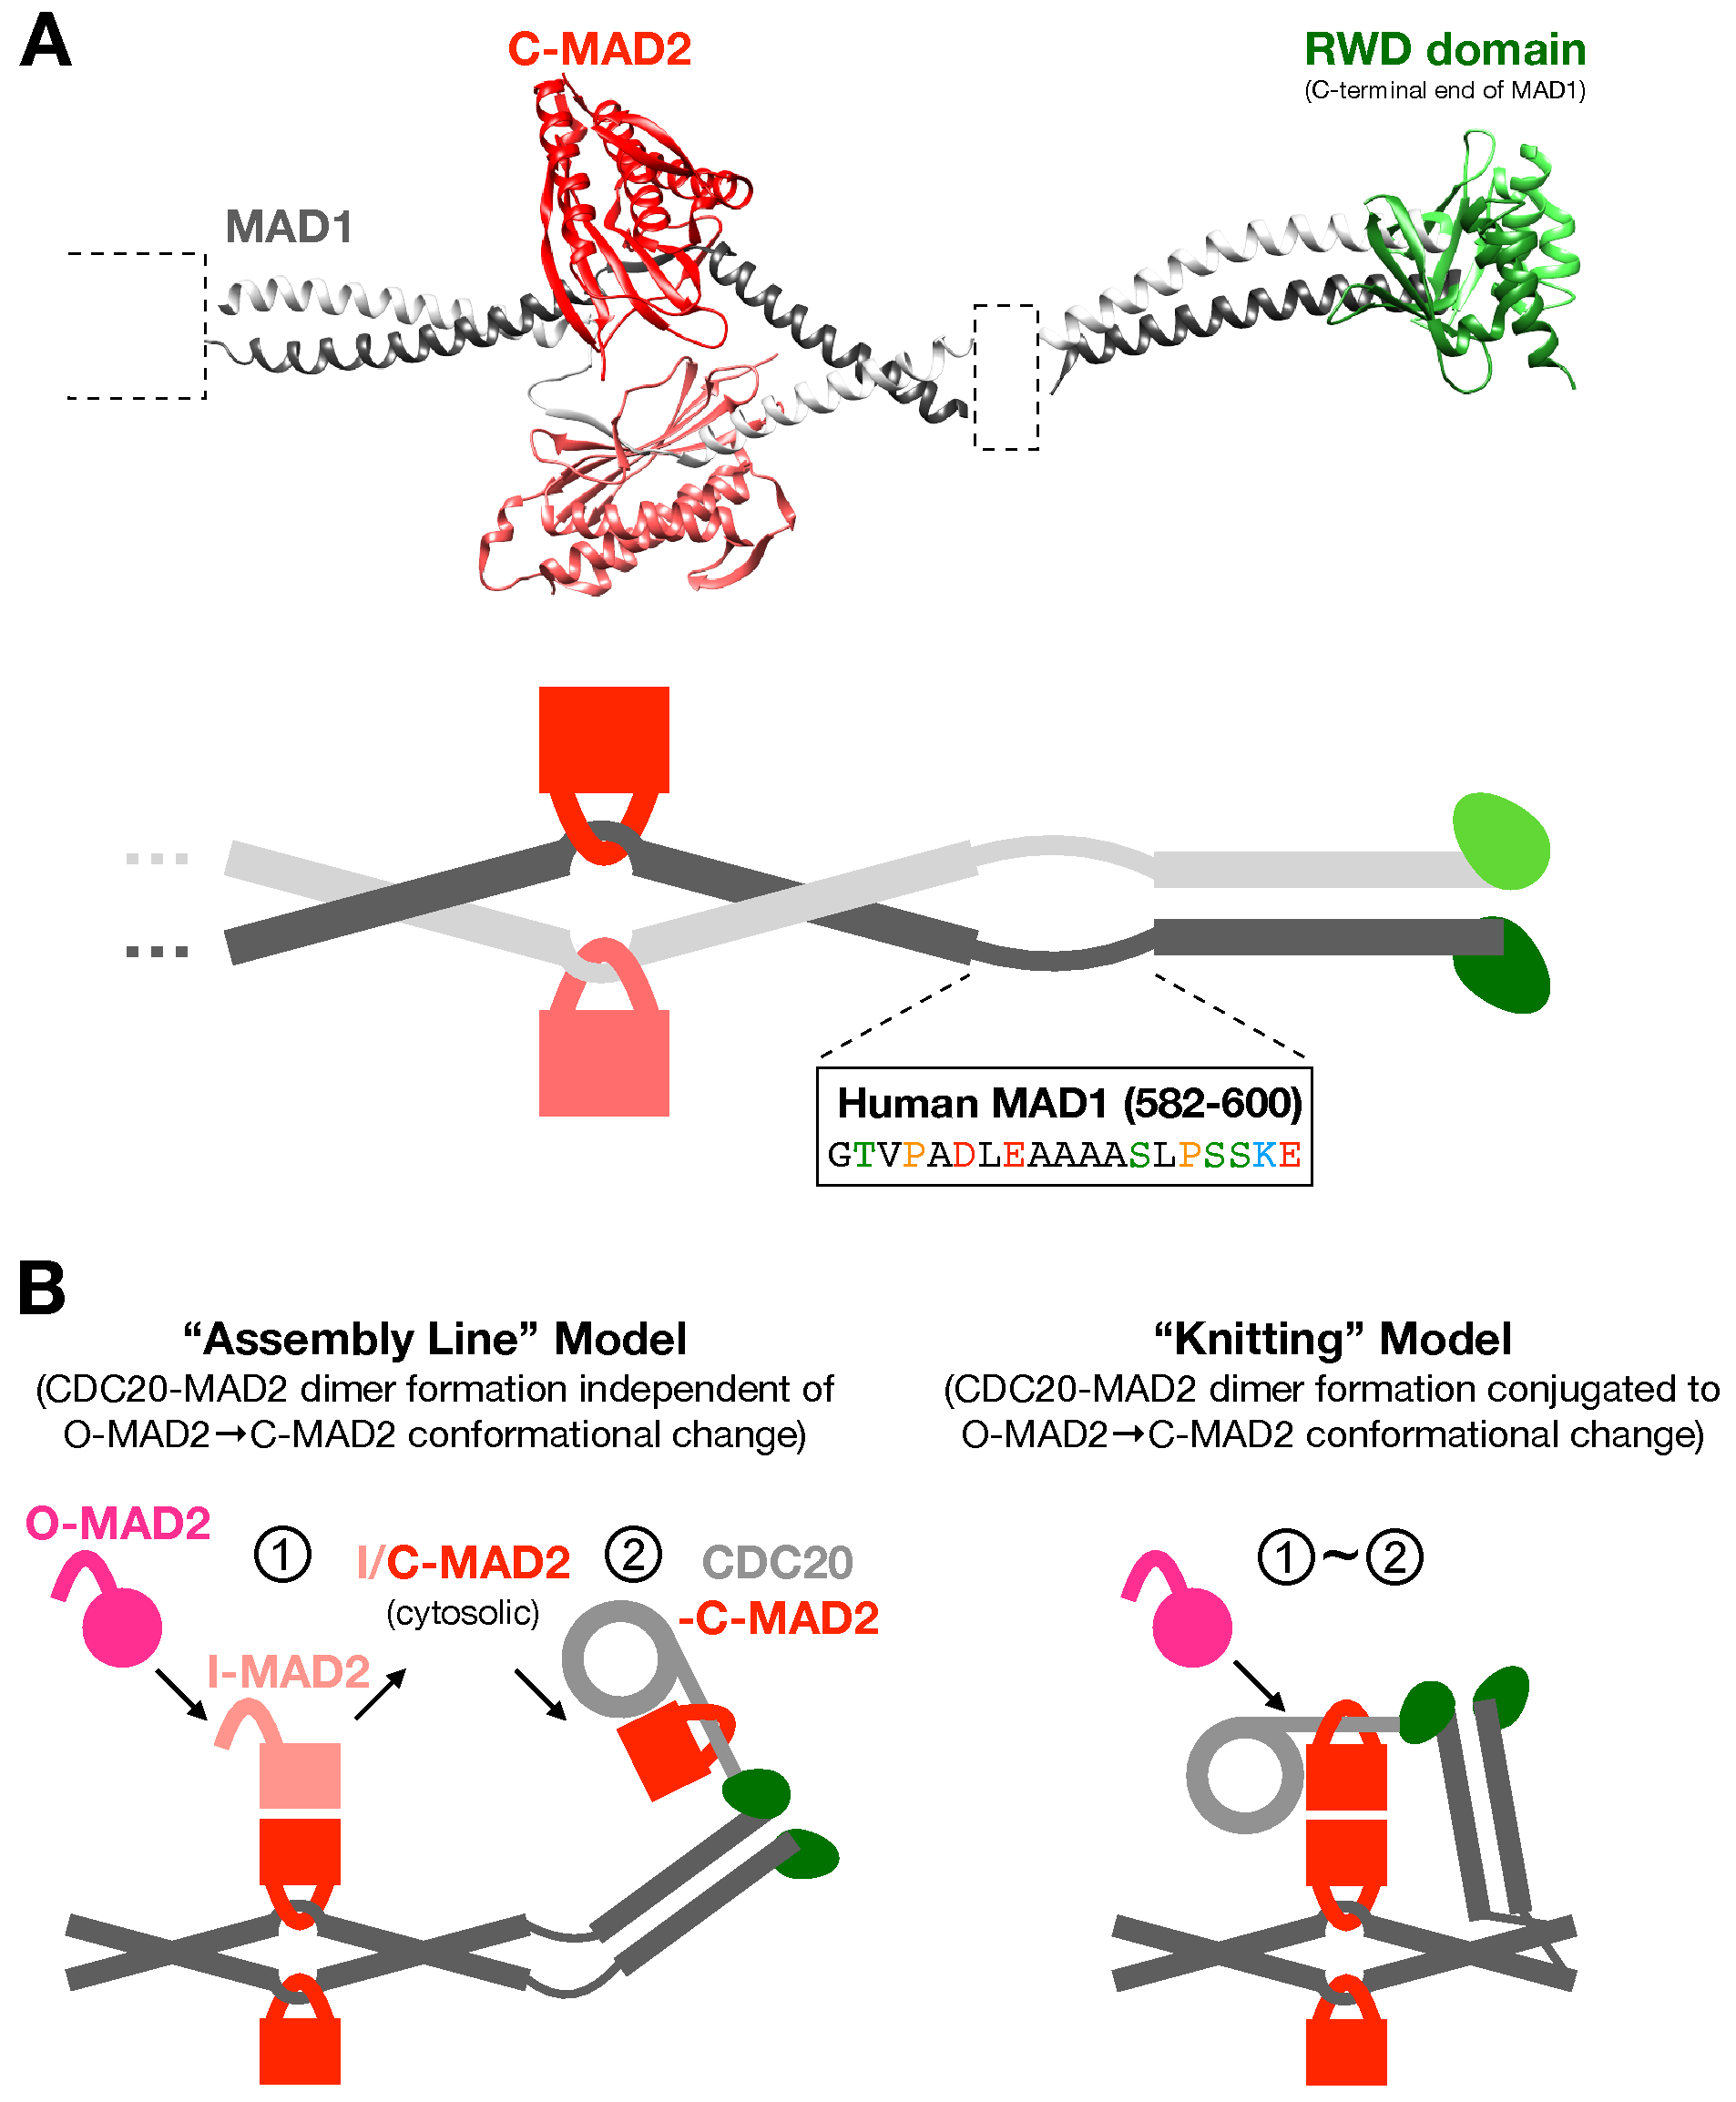
\includegraphics[width=0.75\textwidth]{chapters/figures/MAD1C+KnittingModel.pdf}
    \phantomsubfiglabel{HsMAD1CTerStructure} % subfigure A
    \phantomsubfiglabel{TwoModelCartoons} % subfigure B
    \caption{\textbf{The structure of the \protein{Mad1}-\protein{Mad2} heterotetramer and the two models of the molecular mechanism of \protein{Cdc20}-\protein{Mad2} dimerization.}}
    \noindent\justifying (A) Top panel: the known structure of the \protein{Mad1}-\protein{Mad2} heterotetramer. PDB IDs: 1GO4 (left, \cite{Structure1GO4}), 4DZO (right, \cite{Structure4DZO}). Structures of the N-terminus and the segment spanning a.a. 580--597 are unknown. Various secondary structure prediction algorithms consistently predicted this segment to be a flexible loop (though the predicted starting and ending positions may vary among different algorithms). Bottom panel: a cartoon illustrating the known structure of the \protein{Mad1}-\protein{Mad2} heterotetramer. The color scheme matches the top panel. To distinguish the two \protein{Mad1} proteins [and their C-terminal RWD domains] and the two \protein{Mad2} proteins, slightly different colors are applied. In all cartoons later, both copies will use the same color scheme. The sequence of the loop region (a.a. 582--600) predicted by COILS is shown \cite{LupasCOILS}. Serine/threonine residues are colored green. Proline residues are colored orange. Negatively charged residues are colored red. Lysine residues are colored blue. All cartoons in this chapter are not to scale. (B) The two models of the molecular mechanism of \protein{Cdc20}-\protein{Mad2} dimerization: the "assembly line" model and the "knitting" model.
    \label{MAD1C+KnittingModel}
\end{figure}

\begin{figure}
    \centering
    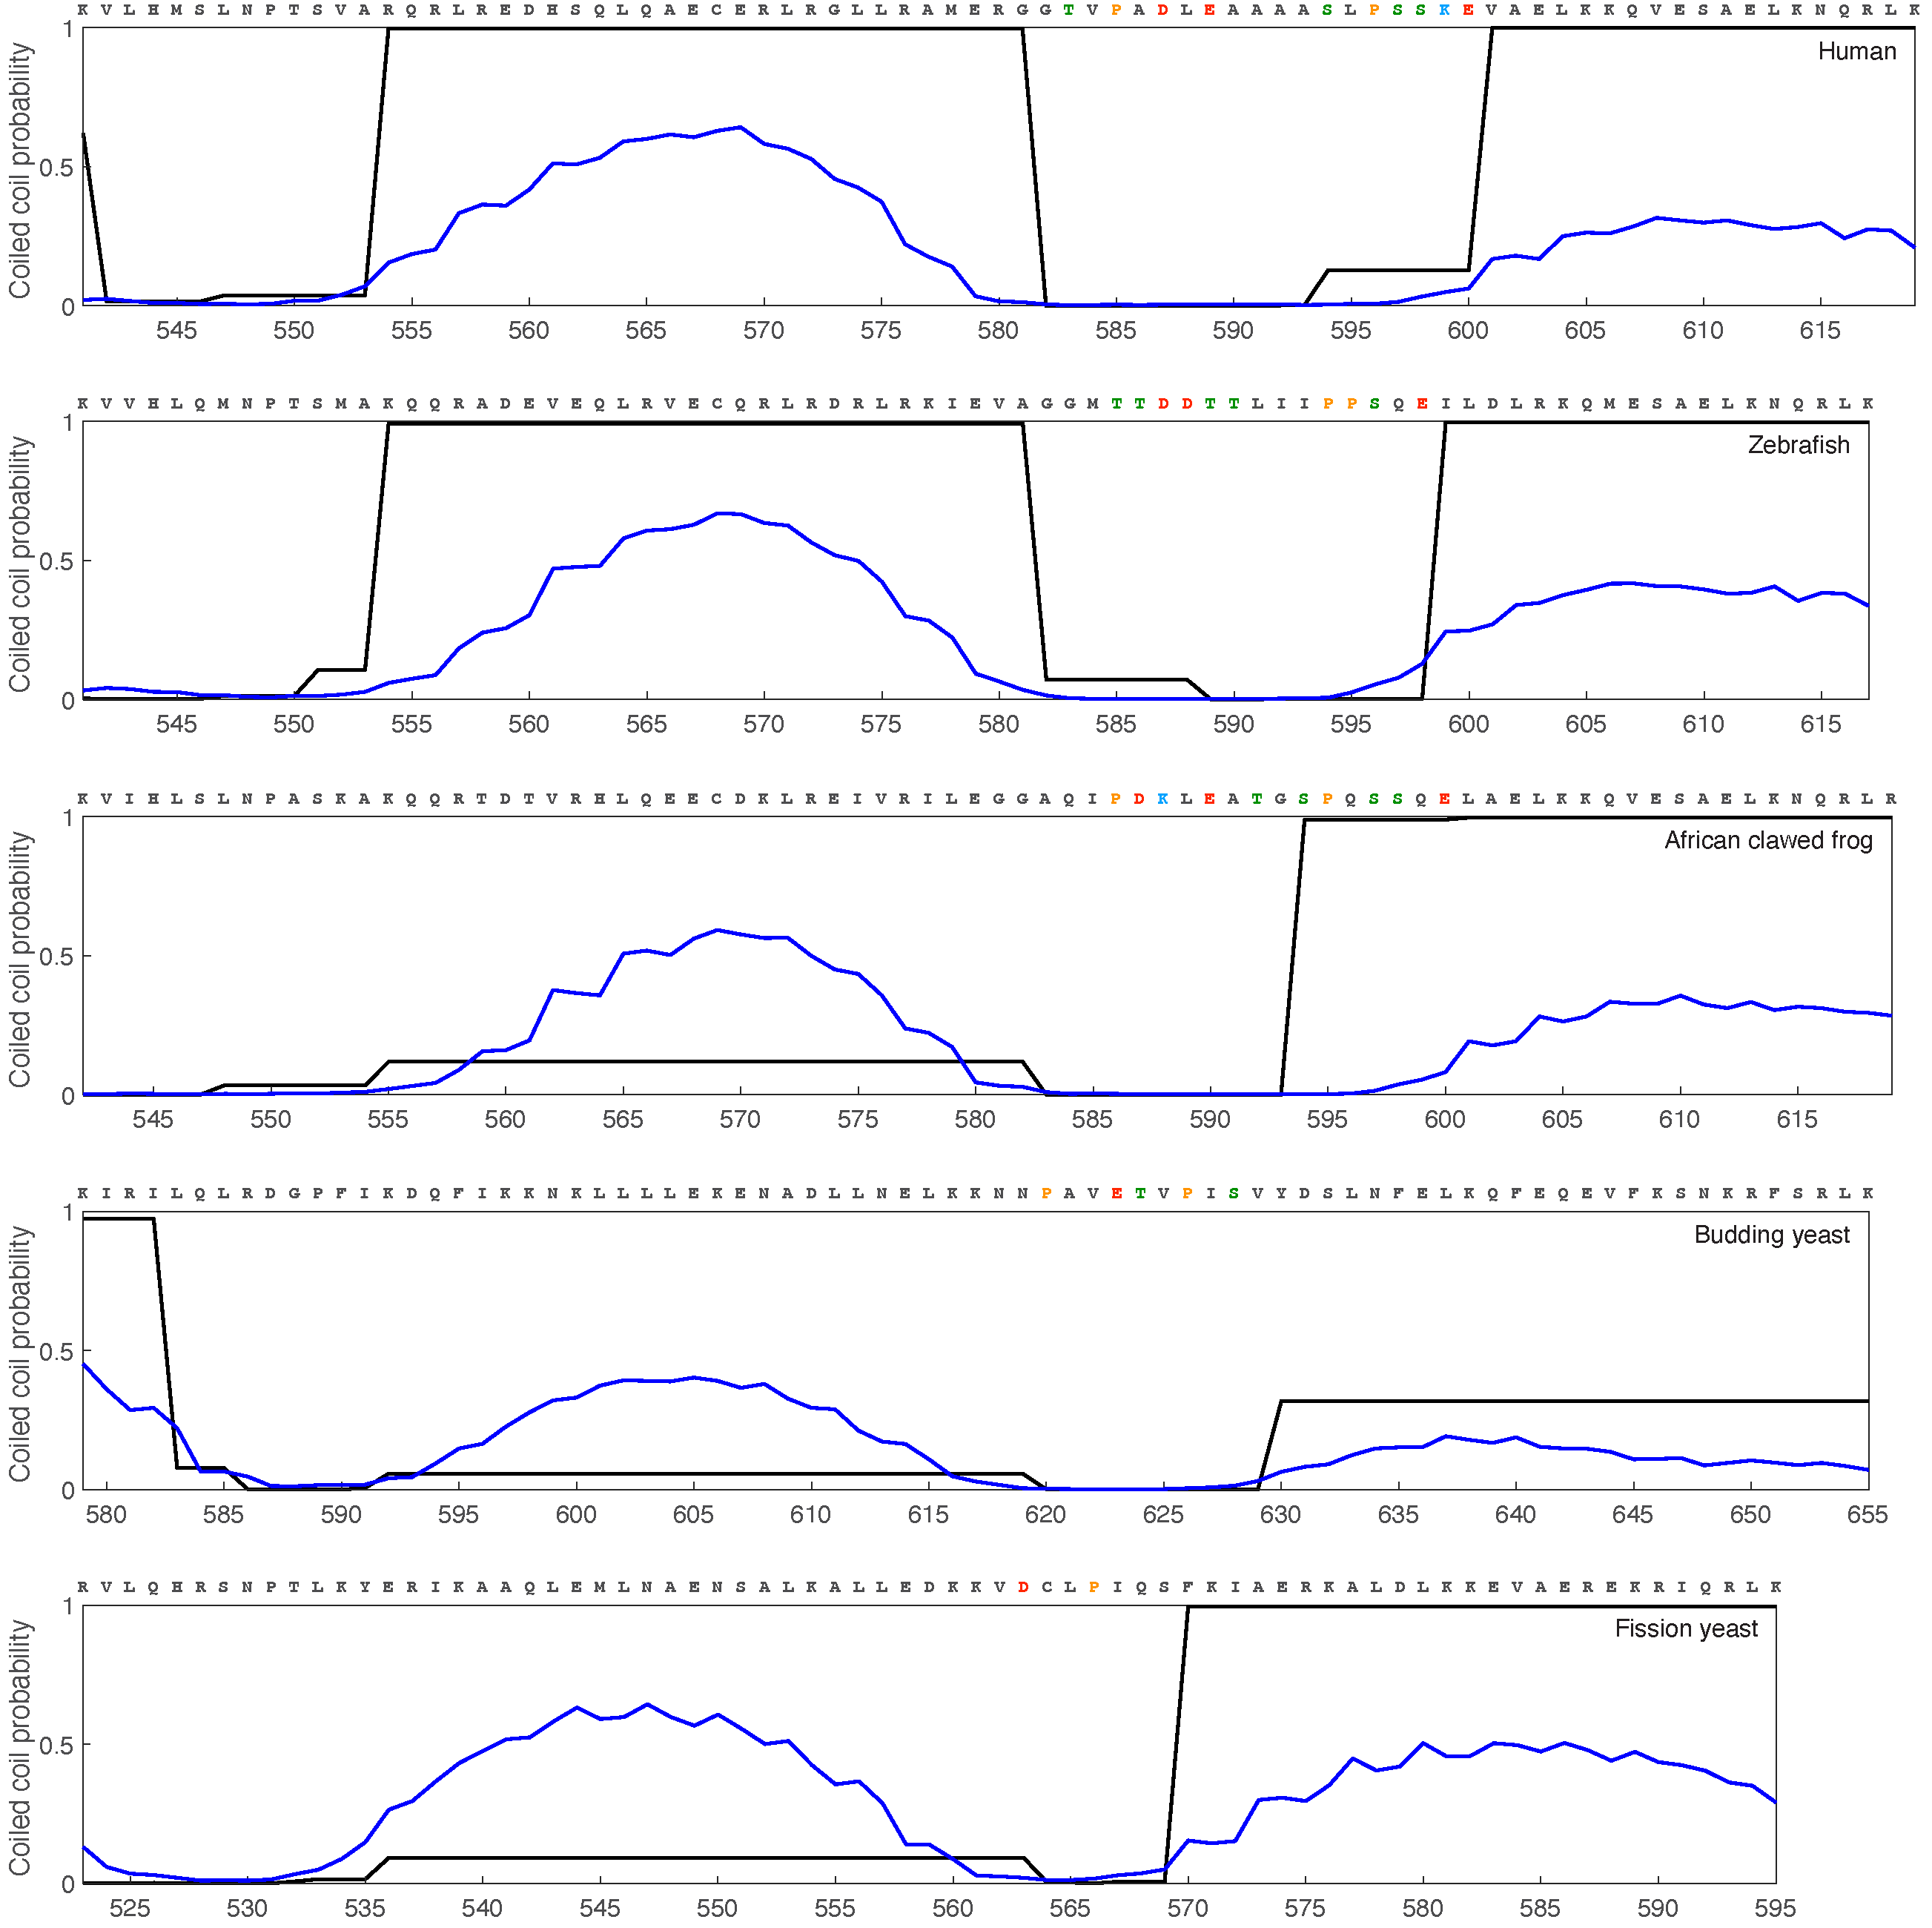
\includegraphics[width=0.98\textwidth]{chapters/figures/MAD1_MIM-RLK_Lupas+DeepCoil2.pdf}
    \caption{\textbf{The secondary structure of \protein{Mad1}'s loop region is well conserved.}}
    \noindent\justifying The primary sequence of \protein{Mad1}'s loop region is not well conserved but the secondary structure is. The figure shows coiled coil predictions by two algorithms (black curves: Lupas' method using a gliding window size of 28 residues \cite{LupasCOILS}; blue curves: raw predicted probabilities by DeepCoil2 \cite{DeepCoil}) on the region spanning from \protein{Mad1}'s MIM (which is also not a coiled coil \cite{Structure1GO4}) to \protein{Mad1}'s consensus RLK motif from \Latin{Homo sapiens} (human), \Latin{Danio rerio} (zebrafish), \Latin{Xenopus Laevis} (African clawed frog), \Latin{Saccharomyces cerevisiae} (budding yeast), and \Latin{Schizosaccharomyces pombe} (fission yeast). The $x$-axis represents the coordinates of residues within \protein{Mad1}. The primary sequences of full-length \protein{Mad1} proteins were supplied as the input, but only probability predictions on this region are shown here. The RLK motif directly binds to \protein{Bub1} \cite{Ji2017eLife, BUB1CD1-MAD1CStructure} and is located within the coiled coil leading to the RWD domain (see the crystal structure on the right in \myref{HsMAD1CTerStructure}). Residues within the putative loop region are colored as in \myref{HsMAD1CTerStructure}.
    \label{MAD1_MIM-RLK_Lupas+DeepCoil2}
\end{figure}

We reason that the ``knitting'' model is more realistic based on many pieces of evidence from previous literature. First, locking cytosolic \protein{Mad2} to its closed conformation inhibited the dimerization between \protein{Cdc20} and \protein{Mad2} and compromised the SAC signaling activity \cite{Ma+Poon2016, Ma+Poon2018, Kim2018}, which can be interpreted by the ``knitting'' model. Second, the binding of \protein{Cdc20} to \protein{Mad1}'s RWD domain is suggested to be important to the SAC signaling activity \cite{Kruse2014, SpMad1, Faesen2017, Ji2017eLife}. One explanation is that the binding may increase the local concentration of \protein{Cdc20}, which is better harnessed by the ``knitting'' model. The anchoring of the basic motif of \protein{Cdc20} to \protein{Mad1}'s RWD domain may even topologically hinder the stringing of \protein{Mad2} that is already in the closed conformation because \protein{Cdc20}'s MIM is between the basic motif and the \textbeta{}-propeller. Third, two recent studies strongly supported the spatio-temporal coupling between \protein{Mad2}'s conformational change and the formation of the \protein{Cdc20}-\protein{Mad2} dimer \cite{BUB1-CDC20-MAD1, Tripartite}.

In this chapter, we intend to prove the "knitting" model by introducing mutations to \protein{Mad1} that theoretically only impair the SAC signaling activity if the "knitting" model is correct. It should be noted that there is a gray area between the two models, given that I-\protein{Mad2} can exist in the solution \cite{I-MAD2}, which may be the fresh \protein{Mad2} conformer coming off the template-based conformational switch, entering the cytosolic pool, and eventually binding to \protein{Cdc20} (becoming C-\protein{Mad2} thereafter). We categorize this situation into the "assembly line" model (also illustrated in \myref{TwoModelCartoons}) because our mutational approach should not impair the SAC signaling activity in this case either (see \myref{LoopDeletionSection}).

\section{The \protein{Mad1}-\protein{Mad2} heterotetramer may adopt a fold-back conformation both \Latin{in vivo} and \Latin{in vitro}}

For the ``knitting'' model to work, the site of \protein{Mad2}'s conformational switch and \protein{Cdc20}'s MIM have to be positioned close enough. According to the crystal structure, the axial length from the MIM to the start of the loop region is about 5--\SI{6}{nm} while the axial length from the end of the loop region to the anchoring point of \protein{Cdc20} is about \SI{7}{nm} \cite{TemplateModel, Ji2017eLife, BUB1-CDC20-MAD1, Structure1GO4, Structure4DZO}. In contrast, if we model the disordered N-terminus of \protein{Cdc20} as a simple 3-D random walk, we can estimate the root-mean-square distance from \protein{Cdc20}'s BOX1 to its MIM (about 90 residues) to be less than \SI{4}{nm}. Due to steric hindrance and restrictions imposed by the Ramachandran plot, such a simple 3-D random walk model is far from realistic. However, even if we apply a more sophisticated worm-like chain model with a persistence length of 3--\SI{4}{\angstrom} \cite{RandomWalk3D-WormLikeChain}, the root-mean-square distance from \protein{Cdc20}'s BOX1 to its MIM is still only about \SI{5}{nm}. These estimations suggest that additional mechanisms may be at work to position the site of \protein{Mad2}'s conformational switch and \protein{Cdc20}'s MIM closely to facilitate the heterodimerization between \protein{Mad2} and \protein{Cdc20}.

One possibility has been suggested in \cite{BUB1-CDC20-MAD1, Tripartite} that the cooperative binding of \protein{Cdc20} to \protein{Mad1}'s RWD domain and \protein{Bub1} helps to unravel the N-terminus of \protein{Cdc20}. Indeed, if the disordered region from \protein{Cdc20}'s BOX1 to its MIM is fully stretched, it will be more than enough for the MIM of the \protein{Cdc20} anchored to \protein{Mad1}'s RWD domain to engage the site of \protein{Mad2}'s conformational switch. However, there are conflicting claims over whether and where \protein{Bub1} directly binds to \protein{Mad1} \cite{Ji2017eLife, BUB1-CDC20-MAD1, BUB1CD1-MAD1CStructure}. If \protein{Bub1}'s conserved domain 1 (CD1, which is also named conserved motif 1 or CM1) directly interacts with \protein{Mad1}'s consensus RLK motif located in \protein{Mad1}'s C-terminal coiled coil \cite{Ji2017eLife, BUB1CD1-MAD1CStructure} (illustrated in \myref{KnittingModel} as the contact between \protein{Bub1} and the C-terminal coiled coil of \protein{Mad1}), the cooperative binding of \protein{Cdc20} to \protein{Bub1} and \protein{Mad1} may not unravel \protein{Cdc20}'s N-terminus because the segment of \protein{Bub1} from CD1 to ABBA-consensus KEN motifs (which bind to \protein{Cdc20} \cite{BUB1-CDC20-MAD1, CDC20-KEN, ABBA}) is also largely disordered (predicted by AlphaFold2 with low confidence; data not shown).

Another possibility has been suggested in \cite{Structure1GO4, SpMad1} that \protein{Mad1} may position the site of \protein{Mad2}'s conformational switch and \protein{Cdc20}'s MIM closely by assuming a fold-back conformation. As mentioned in the previous section, the secondary structure of \protein{Mad1}'s C-terminal loop region is conserved, whose flexibility may enable such fold-back conformation according to the prediction by the ColabFold advanced algorithm (see \myref{MAD1_ColabFoldPrediction}, which is close to the scenario envisioned by \cite{SpMad1}). If we truncate residues 582--600 of human \protein{Mad1}, which removes the flexible loop and fuses the coiled coils upstream and downstream of the loop region (while preserving the original heptad repeat position designation as assigned by Lupas' method \cite{LupasCOILS} as well as DeepCoil2 \cite{DeepCoil}; data not shown), the resulting loop-deleted \protein{Mad1} (henceforth referred to as \protein{Mad1}\textDelta{}L) homodimer can only assume an extended conformation (see \myref{MAD1DeltaL_ColabFoldPrediction}).

\begin{figure}
    \centering
    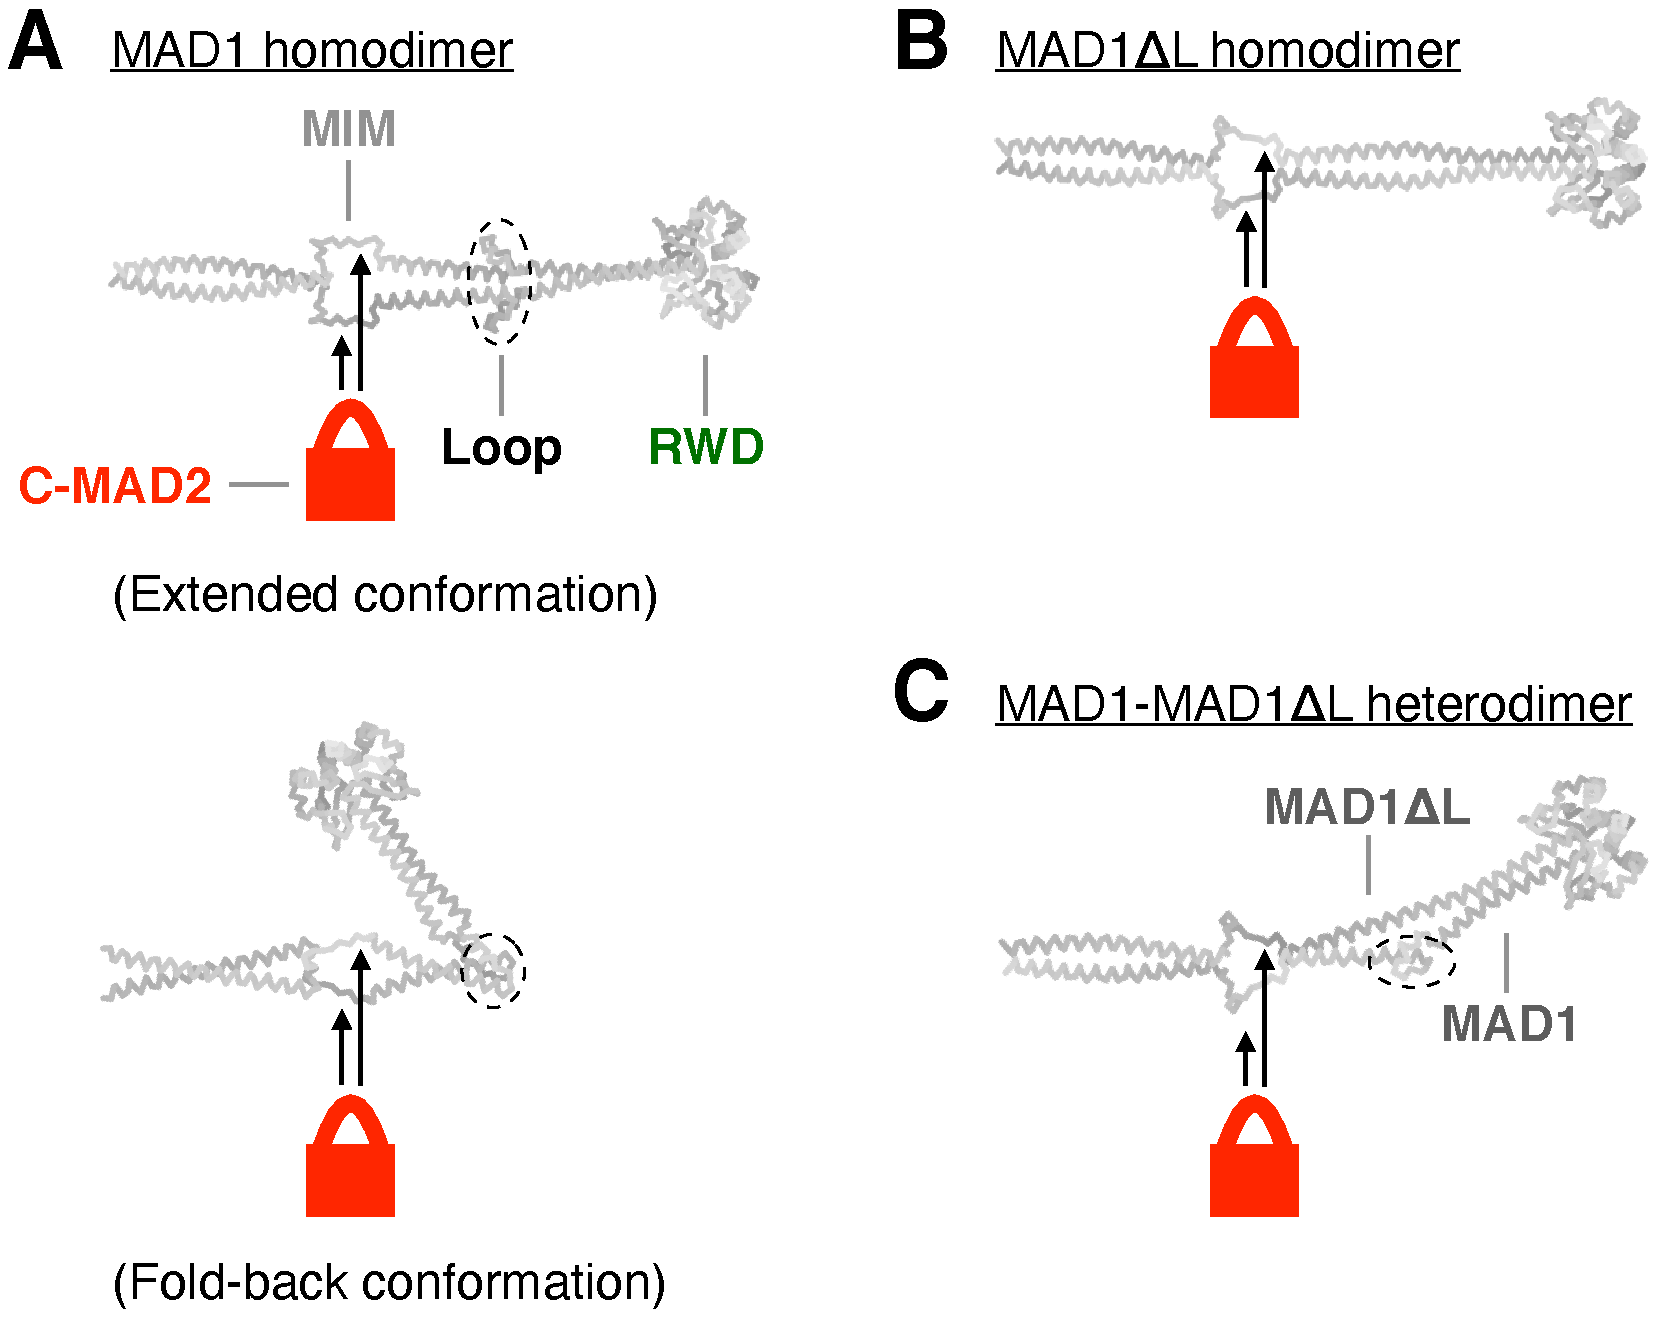
\includegraphics[width=0.85\textwidth]{chapters/figures/ColabFoldPrediction.pdf}
    \phantomsubfiglabel{MAD1_ColabFoldPrediction} % subfigure A
    \phantomsubfiglabel{MAD1DeltaL_ColabFoldPrediction} % subfigure B
    \phantomsubfiglabel{MAD1-MAD1DeltaL_ColabFoldPrediction} % subfigure C
    \caption{\textbf{Representative structures of the C-terminus of the \protein{Mad1} homodimer, the \protein{Mad1}\textDelta{}L homodimer, and the \protein{Mad1}-\protein{Mad1}\textDelta{}L heterodimer were predicted by ColabFold.}}
    \noindent\justifying Representative models (out of five models in total) of the C-terminus of the \protein{Mad1} homodimer (A), the \protein{Mad1}\textDelta{}L homodimer (B), and the \protein{Mad1}-\protein{Mad1}\textDelta{}L heterodimer (C) were predicted by ColabFold using the default parameter settings of ColabFold advanced algorithm. The loop region of wildtype \protein{Mad1} is circled out in (A) and (C). The MIM of \protein{Mad1} where C-\protein{Mad2} binds and the RWD domain at the C-terminal end of \protein{Mad1} where the N-terminal BOX1 of \protein{Cdc20} is anchored are also indicated. The C-terminus of the \protein{Mad1} homodimer may assume a fold-back conformation [see the bottom panel of (A)]. In the predicted structure of the \protein{Mad1}-\protein{Mad1}\textDelta{}L heterodimer, the loop region of the wildtype copy introduces a bulge but the overall conformation is extended. 
    \label{ColabFoldPrediction}
\end{figure}

To confirm such fold-back of \protein{Mad1}, we first noted that about 37\% of purified full-length \protein{Mad1}-\protein{Mad2} heterotetramers do not show distinguishable \protein{Mad1}-MIM-\protein{Mad2} and \protein{Mad1}-RWD domain densities as visualized by electron microscopy using metal shadowing \cite{BUB1-CDC20-MAD1}. This may be explained by that this population of \protein{Mad1}-\protein{Mad2} heterotetramers assumes a fold-back conformation. To further support that the \protein{Mad1} may assume a fold-back conformation \Latin{in vivo}, we resorted to the distance-sensitive FRET measurement. We fused the donor fluorophore mNeonGreen to the C-terminal end of \protein{Mad1} (see \myref{TaggingSACProteins}) and inserted the acceptor fluorophore mScarlet-I into the \textbeta{}5-\textalpha{}C loop of \protein{Mad2} \cite{mSI, beta5-alphaCLoop} (the recombinant protein is henceforth referred to as ``\protein{Mad2}$\wedge$mScarlet-I''; see \myref{MAD2InternalTagging_Strategy}). If the heterotetramer always assumes an extended conformation, the distance between the donor and acceptor will be larger than \SI{10}{nm}, which allows no or minimal FRET between the donor \protein{Mad1}-mNG and the acceptor \protein{Mad2}$\wedge$mScarlet-I. However, if the heterotetramer may assume a fold-back conformation, the distance between the donor and acceptor may be reduced to allow for FRET between the donor and the acceptor.

\begin{figure}
    \centering
    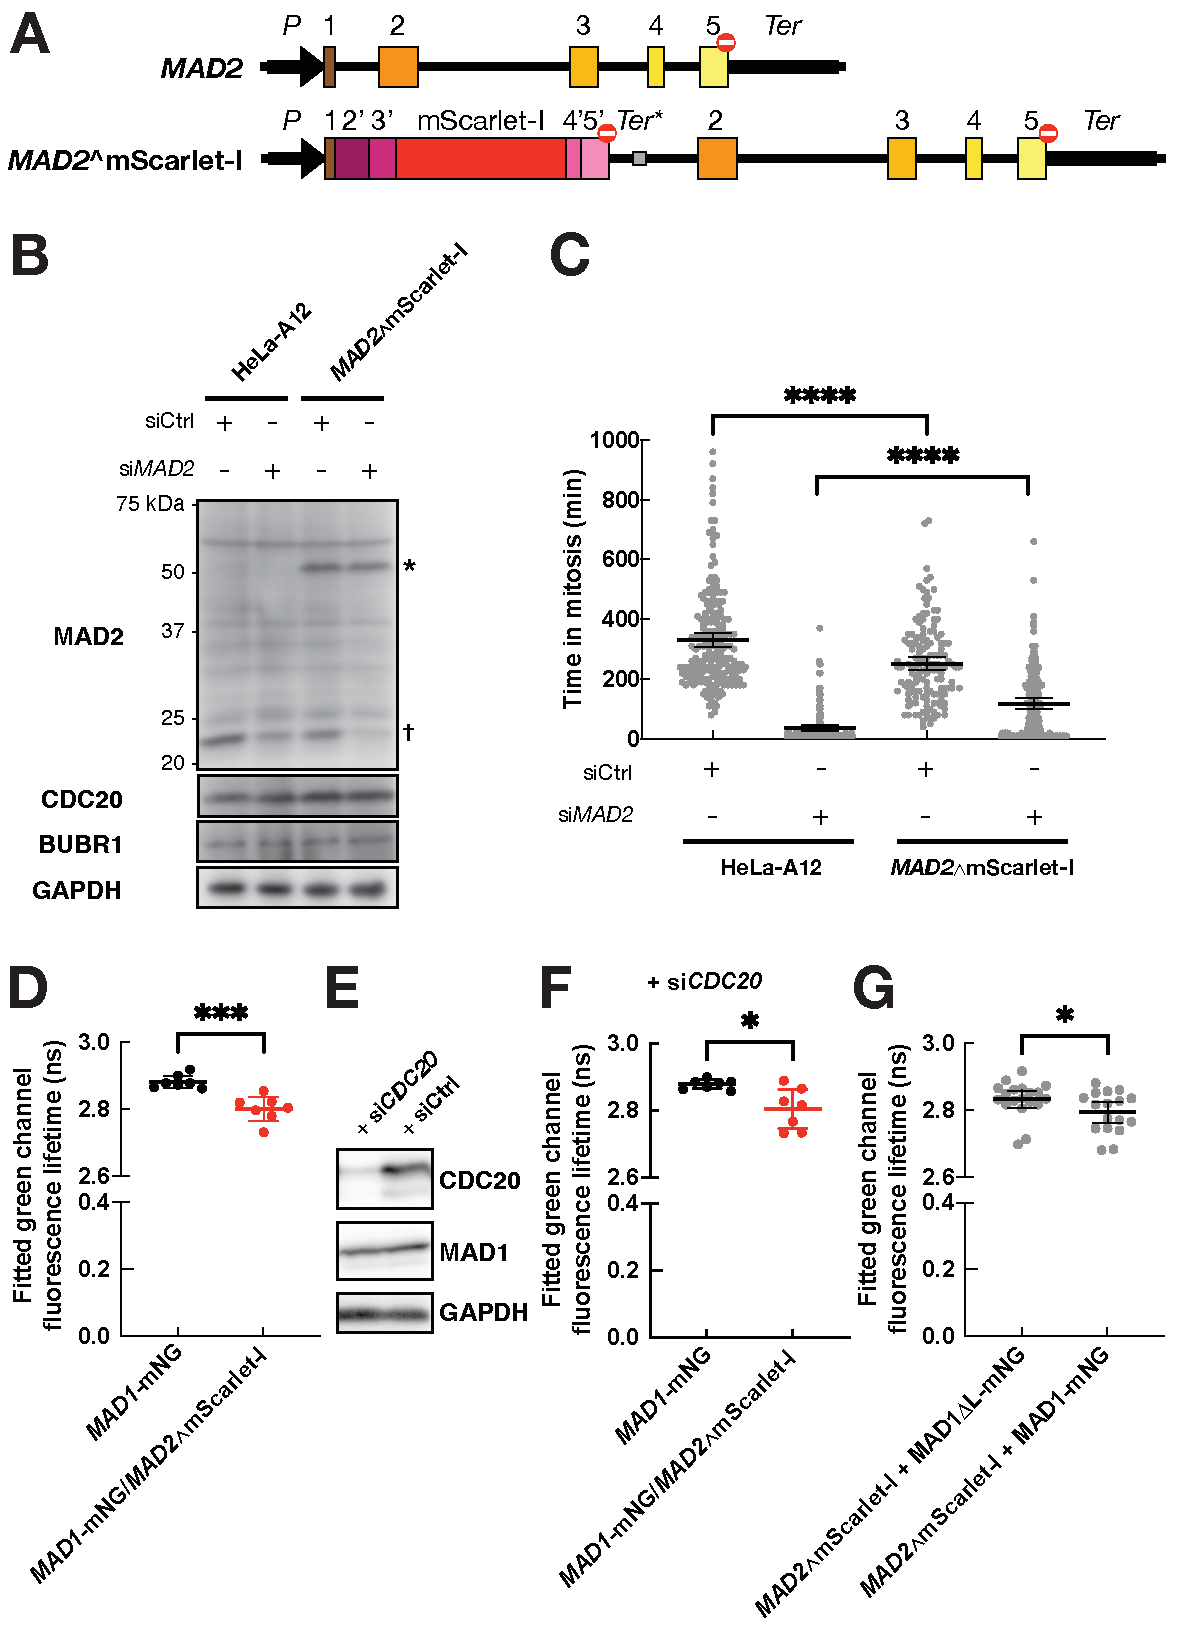
\includegraphics[width=0.91\textwidth]{chapters/figures/InternallyTaggedMAD2+NPCFLIM.pdf}
    \phantomsubfiglabel{MAD2InternalTagging_Strategy} % subfigure A
    \phantomsubfiglabel{MAD2InternalTagging_WB} % subfigure B
    \phantomsubfiglabel{MAD2InternalTagging_SACActivity} % subfigure C
    \phantomsubfiglabel{NosiCDC20_FLIM} % subfigure D
    \phantomsubfiglabel{siCDC20_WB} % subfigure E
    \phantomsubfiglabel{siCDC20_FLIM} % subfigure F
    \caption{\textbf{The observation of FRET between \protein{Mad1}-mNG and \protein{Mad2}$\wedge$mScarlet-I at the interphase/prophase NPC suggested that \protein{Mad1}-\protein{Mad2} heterotetramers may assume a fold-back conformation \Latin{in vivo}.}}
    \label{InternallyTaggedMAD2+NPCFLIM}
\end{figure}
\begin{figure}
    \noindent\justifying \textbf{(Caption of \myref{InternallyTaggedMAD2+NPCFLIM} continued from a previous page)} (A) Diagram of the endogenous gene{Mad2} allele and the genome-edited \gene{Mad2}$\wedge$mScarlet-I allele. Boxes 1--5 represent the exons. The regions between these boxes represent the introns. Boxes 2'--5' encode the same peptides as boxes 2--5 respectively, with the introduction of certain silence mutations that make the recombinant \protein{Mad2}$\wedge$mScarlet-I resistant to si\gene{Mad2}. The black ``\textit{P}'' arrow represents the promoter and the 5'-UTR. The black ``\textit{Ter}'' bar represents the 3'-UTR and the polyadenylation signal. The gray ``\textit{Ter}*'' bar represents the polyadenylation signal of rabbit \textbeta{}-globin. The red stop signs represent stop codons. The sequence of the \gene{Mad2}$\wedge$mScarlet-I allele was confirmed by genotyping and Sanger sequencing (data not shown). (B) Immunoblotting showed that \protein{Mad2}$\wedge$mScarlet-I (labeled by an asterisk, with an expected molecular weight of \SI{51.0}{kDa}) was correctly expressed in the heterozygous \gene{Mad2}$\wedge$mScarlet-I HeLa-A12 cell line and was resistant against si\gene{Mad2}. As a comparison, wildtype \protein{Mad2} (labeled by a cruciform with a molecular weight of \SI{23.5}{kDa}) was effectively knocked down by si\gene{Mad2}. The immunoblot against GAPDH served as the loading control. (C) Unsynchronized cells were treated with respective siRNAs for one day, treated with \SI{50}{nM} nocodazole. Each gray dot represents a cell. The total number of cells in each group $N > 140$. Mean values $\pm 95\%$ confidence intervals are overlaid. Unpaired $t$-tests with Welch's correction were performed in Prism 9. Results are representative of two independent experiments. (D) The average lifetime of \protein{Mad1}-mNG in the \gene{Mad1}-mNG or the \gene{Mad1}-mNG/\gene{Mad2}$\wedge$mScarlet-I double genome-edited HeLa-A12 cell  line using a two-component exponential decay to fit the raw data of FLIM. Each dot represents a single cell. Mean values $\pm 95\%$ confidence intervals are overlaid. The total number of cells in each group $N = 7$. Results are representative of two independent experiments. Unpaired $t$-tests with Welch's correction were performed in Prism 9. (E) Unsynchronized HeLa-A12 cells were treated with si\gene{Cdc20} or a control siRNA for \SI{2}{d} and probed for \protein{Cdc20}, \protein{Mad1}, and GAPDH (loading control). (F) Same as (D), except that cells were treated with si\gene{Cdc20} as in (E).
\end{figure}

We confirmed the expression of full-length \protein{Mad2}$\wedge$mScarlet-I in the heterozygous \gene{Mad2}$\wedge$mScarlet-I genome-edited HeLa-A12 cell line (see \myref{MAD2InternalTagging_WB}), wherein the expression level of either \protein{BubR1} or \protein{Cdc20} was not affected. \protein{Mad2}$\wedge$mScarlet-I could support a certain degree of the SAC signaling activity when the endogenous wildtype \protein{Mad2} was knocked down (see \myref{MAD2InternalTagging_SACActivity}). Using fluorescence lifetime imaging microscopy (FLIM), we quantified a FRET efficiency of about 3\% between \protein{Mad1}-mNG and \protein{Mad2}$\wedge$mScarlet-I at the interphase/prophase NPC in the heterozygous \gene{Mad1}-mNG, \gene{Mad2}$\wedge$mScarlet-I genome-edited HeLa-A12 cell line (see \myref{NosiCDC20_FLIM}). We chose to measure FRET at the interphase/prophase NPC to facilitate data collection by the line-scanning confocal microscope and to avoid the potential intermolecular FRET between a donor from one \protein{Mad1}-\protein{Mad2} heterotetramer and an acceptor from another nearby heterotetramer at the corona of a signaling kinetochore. This FRET persisted even when \gene{Cdc20} was knocked down by RNAi (see \myref{siCDC20_WB,siCDC20_FLIM}), which indicates that this FRET does not depend on \protein{Mad1}'s catalytic role but is rather intrinsic to the structural characteristics of the \protein{Mad1}-\protein{Mad2} heterotetramer. Although we still cannot completely rule out potential intermolecular FRET, we confirmed the existence of the anticipated FRET that may result from the fold-back of \protein{Mad1} \Latin{in vivo}.

\section{\protein{Mad1}'s loop region is important to the SAC signaling activity \Latin{in vivo}}
\label{LoopDeletionSection}

\section{The function of \protein{Mad1}'s loop region does not depend on the potential phosphorylation of any serine or threonine residues within it}

\section{The structural flexibility of \protein{Mad1} enabled by its loop region facilitates the ``knitting'' of the MCC}
\label{FinalKnittingModel}

% BUB1 positioning: \cite{Ji2017eLife, BUB1-CDC20-MAD1, BUB1CD1-MAD1CStructure, CDC20-KEN, ABBA}
% First, \protein{Mad1} in its fold-back conformation physically positions the MIM of \protein{Cdc20} and \protein{Mad2} closely, facilitating their association. Second, the cooperative interaction between the scaffold protein \protein{Mad1} in its fold-back conformation and \protein{Cdc20}-\protein{Mad2} favors the formation of the \protein{Mad1}RWD-\protein{Cdc20}-\protein{Mad2}-\protein{Mad1}MIM complex. Third, the extended conformation breaks such avidity binding and promotes the release of \protein{Cdc20}-\protein{Mad2} into the cytosol. However, future studies are needed to fill in the gaps between our current experimental evidence and the ``knitting'' model.

\section{Discussions}
\label{Chapter4Discussions}

% MAD1 exposes CDC20-MIM from masking?

% Two possibilities of how CDC20 MIM is brought to close proximity with MAD2 are not mutually exclusive.

In this study, we showed for the first time that the \protein{Mad1}-\protein{Mad2} heterotetramer can assume a fold-back conformation both \Latin{in vitro} and \Latin{in vivo}. Our preliminary data indicate that the structural flexibility is enabled by a flexible loop in the C-terminus of \protein{Mad1}, whose secondary structure is conserved. This loop region is important to the SAC signaling activity both \Latin{in vitro} and \Latin{in vivo} and its role does not depend on any potential phospho-regulation of the serine/threonine residues within. We proposed a ``knitting'' model to explain how the structural flexibility of \protein{Mad1}-\protein{Mad2} heterotetramer may facilitate the spatio-temporal coupling between \protein{Mad2}'s conformational change and \protein{Cdc20}-\protein{Mad2} dimerization. It should be noted that even in the absence of \protein{Cdc20}, O-\protein{Mad2} can bind to the \protein{Mad1}-\protein{Mad2} heterotetramer, complete the conformational switch, and dissociate as C-\protein{Mad2} \Latin{in vitro} \cite{Yang2008}. Finding out whether \protein{Cdc20} increases the rate of \protein{Mad2}'s conformational switch will help us further understand the mechanism of the catalysis.

\protein{Mad1} has a long half-life under normal conditions \cite{MAD1MAD2Half-life}. And like \protein{Bub1} \cite{Raaijmakers2018, RZZ-MAD1vsBUB1-MAD1_2018, siROD_Zhang2019}, even a small pool of \protein{Mad1} (at less than 10\% on average of its physiological concentration in our knockdown experiments) can maintain a considerable level of SAC signaling activity in nocodazole-treated cells. Future studies should consider combining RNAi (or induced knockout of \gene{Mad1}) with induced acute degradation of \protein{Mad1} proteins to reduce the contribution of the remaining endogenous \protein{Mad1} homodimer to the SAC signaling activity and to minimize the chance of heterodimerization between the remaining endogenous \protein{Mad1} and the rescuing \protein{Mad1} variants in such knockdown-rescue experiments. %(AID, Trim-Away, etc. for such a nuclear protein during the interphase/prophase).

Given the critical role of \protein{Mad1}'s structural flexibility enabled by its loop region, it would be interesting to replace the flexible loop with a turn to lock \protein{Mad1} in the fold-back conformation and see how the SAC signaling activity is affected. Another way to advance our understanding is to investigate whether the two pools of \protein{Mad1} (adopting either the fold-back or extended conformation) inter-convert at a physiologically meaningful rate in the cell using single-molecular approaches. Even though the two proline residues (P585 and P596) in \protein{Mad1}’s loop region may be important to the SAC signaling activity \Latin{in vivo}, no \protein{Mad1}-interacting protein with peptidylprolyl cis-trans isomerase activity has been identified in the PrePPI database using the gene ontology enrichment analysis tool from the PANTHER Classification System as of March 2022 \cite{PrePPI, PANTHER}. Additionally, it might be worth finding out whether the equilibrium between the two conformations in the cell is the same as purified \protein{Mad1}-\protein{Mad2} heterotetramer \Latin{in vitro}, which would tell us if the conformation distribution is under active regulation in the cell that costs energy \cite{MAD2Dynamics}. % However, this does not completely rule out the possibility because the interaction between \protein{Mad1} and a peptidylprolyl isomerase might be transient.

Two missense variants (D587N and A593V) related to \protein{Mad1}’s loop region were recorded in the Genomic Data Commons Data Portal as of March 2022 \cite{GDC}, but the impact of both point mutations is predicted to be benign. Therefore, the physiological impact of potential mutations in \protein{Mad1}’s loop region at the organism level is unclear. It would be interesting to see the physiological impact of introducing point mutations (for example, the multiple proline residues) in \protein{Mad1}’s loop region in various model systems.

In addition to \protein{Cdc20}, closed \protein{Mad2} also interacts with many other proteins (including \protein{Mad1}, \protein{Sgo2} \cite{SGO2-MAD2}, the insulin receptor \cite{MCC_IREndocytosis}, and \protein{Kif20a} \cite{KIF20A-MAD2}), likely by a similar ``safety belt'' mechanism \cite{Structure1GO4}. One question that comes up naturally is whether the same catalytic mechanism (the spatio-temporal coupling between \protein{Mad2}'s conformational change and \protein{Cdc20}-\protein{Mad2} dimerization) similarly applies to how \protein{Mad2} binds to other proteins (or even more generally, whether the same catalytic mechanism applies to how other HORMA domain proteins bind to other proteins \cite{HORMAReview})? One interesting finding is that the S214A mutation in human \protein{Mad1} impairs the homodimerization of \protein{Mad1} as well as the interaction between \protein{Mad1} and \protein{Mad2} \cite{ATMPhosphorylatesMad1S214}. S214A is unlikely to affect the binding of \protein{Mad2} to \protein{Mad1}'s MIM directly, given the structure of the \protein{Mad1}-\protein{Mad2} heterotetramer \cite{Structure1GO4} and the fact that S214 and MIM are over 300 amino acids apart. This suggested that the homodimerization of \protein{Mad1} might facilitate the binding of \protein{Mad2} to \protein{Mad1}. One possibility is that one copy of \protein{Mad1} may trans-activate the binding of \protein{Mad2} to the other copy of \protein{Mad1} in the \protein{Mad1}-\protein{Mad2} heterotetramer. Future experiments are needed to elucidate the structural and catalytic basis of how \protein{Mad2} ``buckles up'' its binding partners, which may unveil how \protein{Mad2} regulates mitosis beyond the assembly of the MCC \cite{Separase-SGO2-MAD2, KIF20A-MAD2}. % is it over-reading?

\Latin{In vitro} reconstitution data from our collaborators suggested that the critical role of the flexibility of \protein{Mad1} in scaffolding the spatio-temporal coupling between \protein{Mad2}'s conformational change and \protein{Cdc20}-\protein{Mad2} dimerization relies on \protein{Bub1}. In the absence of \protein{Bub1} in the reactions, the formation rates of \protein{Cdc20}-\protein{Mad2} were the same for both \protein{Mad1} and \protein{Mad1}\textDelta{}L (data not shown). However, it is known that the assembly of the MCC also occurs during the interphase and prophase \cite{PremitoticMCC}. There has been no report on \protein{Bub1}'s localization at the NPC where the \protein{Mad1}-\protein{Mad2} heterotetramer is predominantly localized during the interphase and prophase. Therefore, either the flexibility of \protein{Mad1} alone scaffolds the coupling at the NPC or there may be a nucleoporin that functions similarly to \protein{Bub1}. Interestingly, the nuclear basket protein \protein{Tpr}, which directly associates with the \protein{Mad1}-\protein{Mad2} heterotetramer during the interphase and prophase \cite{TPR-MAD1_Lee2008}, is predicted to bind to \protein{Cdc20} directly in the PrePPI database \cite{PrePPI}. Future studies should look into how the \protein{Mad1}-\protein{Mad2} heterotetramer may catalyze the formation of the \protein{Cdc20}-\protein{Mad2} dimer at the NPC during the interphase and prophase.

\section{Materials and Methods}
For methods of cell culture and Cre-\bacterialgene{lox} RMCE, see \myref{CellCulture+RMCE_Methods}. Time-lapse live-cell imaging was performed on an ImageXpress Nano Automated Imaging System as described in \myref{chpt3ImagingMethods}. Wide-field, $z$-stack fluorescence imaging used in the quantification of localization of \protein{Mad1}(WT/\textDelta{}L)-mNG and \protein{Mad2}$\wedge$mScarlet-I at signaling kinetochores was also as described in \myref{chpt3ImagingMethods}.

\subsection{Generating the \gene{Mad2}$\wedge$mScarlet-I genome-edited HeLa-A12 cell line}

The gRNA used in the integration of the coding sequence of \protein{Mad2}$\wedge$mScarlet-I (intron-free, stop codon-containing, and si\gene{Mad2}-resistant by the introduction of silent mutations) and the polyadenylation signal of rabbit \textbeta{}-globin with the first exon of the endogenous \gene{Mad2} gene 
% ? see \myref
was \Oligo{ucgcgcaggccaauauaucg}. Synthesis of the sgRNA and assembly of the \Latin{Sp}Cas9-sgRNA RNP complex were as described in \myref{CRISPRMethods}. Plain or \gene{Mad1}-mNG genome-edited HeLa-A12 cell lines were co-transfected with the RNP complex and linearized pCC35, sorted, and validated as described in \myref{CRISPRMethods}. A successfully edited \gene{Mad2}$\wedge$mScarlet-I allele encodes an internally-tagged \protein{Mad2} protein, wherein wildtype \protein{Mad2} and mScarlet-I are separated by short flexible linkers (\Peptide{AGSGSGGAS} between the S114 of \protein{Mad2} and the N-terminus of mScarlet-I; \Peptide{GTGAGSA} between the C-terminus of mScarlet-I and the A115 of \protein{Mad2}).

\subsection{RNAi}

The two siRNAs targeting the 3'-UTR of \gene{Mad1} were from \cite{siMAD1-3UTR}. They were applied to unsynchronized cells at a concentration of \SI{40}{nM} each for two days before imaging or collecting cells for immunoblotting unless specified otherwise. The sense-strand sequence of si\gene{Cdc20} was \Oligo{GGAGCUCAUCUCAGGCCAU} \cite{siCDC20}, which was applied at a concentration of \SI{40}{nM} for two days before FLIM or immunoblotting. The sense-strand sequence of si\gene{Mad2} was \Oligo{GGAAGAGUCGGGACCACAGUU} \cite{BubR1MitosisTurnover}, which was applied at a concentration of \SI{40}{nM} for one day before imaging or immunoblotting. Desalted siRNAs modified by double-deoxythymidine overhangs at 3'-ends of both strands were synthesized by Sigma. The AllStars Negative Control siRNA was used as the control. All siRNAs were transfected into the cells via Lipofectamine RNAiMAX following manufacturer’s instructions.

% FLIM

\subsection{Immunoprecipitation using mNeonGreen-Trap}

HeLa-A12 cells integrated with the expression cassette (under the regulation of a TRE) of either mNeonGreen, \protein{Mad1}-mNG, or \protein{Mad1}\textDelta{}L-mNG were induced to express the ectopic recombinant protein by \SI{0.1}{\micro g/ mL} doxycycline (for two days until being harvested) and arrested at mitosis using a thymidine--nocodazole synchronization protocol described in \myref{WBMethods}. Cells were harvested by mitotic shake-off, washed once by PBS, pelleted down by centrifugation at 200--\SI{500}{g} for \SI{3}{min}, snap-frozen in liquid nitrogen, and stored at \SI{-80}{\celsius} before the immunoprecipitation experiment.

On the day of the immunoprecipitation experiment, cells were thawed on ice and lysed in the IP lysis buffer [\SI{75}{mM} HEPES-HCl (pH 7.5 at \SI{4}{\celsius}), \SI{150}{mM} KCl, 10\% (by volume) glycerol, \SI{1.5}{mM} \ch{MgCl2}, \SI{1.5}{mM} EGTA, and 1\% (by mass) CHAPS, a zwitterionic detergent] supplemented before usage with \SI{1}{mM} PMSF, the cOmplete\texttrademark{} EDTA-free Protease Inhibitor Cocktail, PhosSTOP\texttrademark{} (Roche), and a phosphatase inhibitor cocktail (\SI{1}{mM} \ch{Na4P2O7}, \SI{0.1}{mM} \ch{Na3VO4}, \SI{5}{mM} NaF, and \SI{2}{mM} sodium \textbeta-glycerophosphate). For \SI{1}{mg} of wet cell pellet, \SI{40}{\micro L} of \SI{4}{\celsius} IP lysis buffer was added, yielding a total protein concentration of about \SI{5.6}{mg/mL} (if cells were lysed completely). Resuspended cells were rotated for \SI{30}{min} at \SI{4}{\celsius} and then centrifuged at \SI{18000}{g} for \SI{20}{min} at \SI{4}{\celsius}. \SI{600}{\micro L} of supernatant was subsequently cleared by \SI{50}{\micro L} of equilibrated control agarose beads (ChromoTek) to reduce non-specific bindings, rotating for \SI{45}{min} at \SI{4}{\celsius}. The mixture was centrifuged at \SI{2000}{g} for \SI{5}{min} at \SI{4}{\celsius}. \SI{580}{\micro L} of pre-cleared supernatant was then mixed with \SI{30}{\micro L} of equilibrated mNeonGreen-Trap Agarose (nta-20, ChromoTek) and rotated for \SI{1}{h} at \SI{4}{\celsius}. These beads were then pelleted down at \SI{2000}{g} for \SI{5}{min} at \SI{4}{\celsius} and the supernatant was removed. The beads were further washed for four times (rotated for \SI{5}{min} at \SI{4}{\celsius} and then pelleted down at \SI{2000}{g} for \SI{5}{min} at \SI{4}{\celsius}) using \SI{1}{mL} of the IP wash buffer [\SI{75}{mM} HEPES-HCl (pH 7.5 at \SI{4}{\celsius}), \SI{150}{mM} KCl, 10\% (by volume) glycerol, \SI{1.5}{mM} \ch{MgCl2}, and \SI{1.5}{mM} EGTA] each time. The beads were transferred to a fresh tube before the last wash to avoid the non-specific binding of proteins to the wall of the tube. Finally, $2\times$ Laemmli buffer supplemented with \textbeta-mercaptoethanol was added to the beads. Samples were boiled in a boiling water bath for \SI{10}{min} before being subjected to SDS-PAGE and immunoblotting analysis.

% Immunoblotting